\section{Experimental Results and Model Fitting}
\label{sec:fitting_the_model}


This section describes strategies and results for fitting the PDE model to data for the Hamamatsu (HPK) VUV4 and FBK VUV-HD SiPMs. We detail the most robust results and impact of modified fitting strategies. The temperature dependent photoabsorption correction (\autoref{model:temp}) is applied to the default optical dataset, and all absolute PDE measurements are performed above 350~nm where the quantum yield is unity \cite{Lewis_2025_qy}.

\subsection{Fitting method}
\label{sec:fit_sequential}
Subsets of the experimental data can constrain PDE parameters in a sequential and fairly independent manner. Junction geometries and corresponding avalanche initiation is separable using wavelengths where either $W_p=0$ or $W_n=0$. Oxide thickness and surface properties can be probed using angular efficiency and/or specular reflectivity. Measurements are tabulated in \autoref{tab:fitting_procedure}.

\begin{table}[ht]
\centering
\caption{\label{tab:fitting_procedure}
Summary of fitting procedures which can constrain different parameters/regions of the PDE model. For thin oxides, reflectivity vs angle is less powerful than vs wavelength.
}
{\smallskip
\footnotesize
\renewcommand{\arraystretch}{2.0}  % Default is 1.0
\begin{tabular}{|c|c|c|c|c|c|}
\hline
\textbf{Order} & \textbf{Physics} & \makecell{\textbf{Constrained} \\ \textbf{parameter}} & \makecell{\textbf{Measurement}} & \textbf{Equation (PDE or other)} & \makecell{\textbf{Data}\\\textbf{Source}} \\ 
\hline
1 & \makecell{Optics \\(thin oxide)} & $\tox$ & UV reflectivity; $\lambda$ & $R(\lambda; \tox)$ (\autoref{eq:Ref_wave}) & \cite{sipmRef_nexo_guofu} \\
\hline
1 & \makecell{Optics \\(thick oxide)} & $\tox$ & Relative $PDE(\theta)$ & \makecell{\rule{0pt}{2ex} $PDE(\theta) \approx PDE(0)~ \frac{T(\theta)}{T(0)}$ \rule{0pt}{2ex}} & \scriptsize{this work}\\
\hline
2 & p depth & $d_p^*$ & \makecell{\scriptsize UV $PDE(\lambda)$\\$\lambda \lesssim 420$~nm, high $V$} & $FF \cdot T \cdot \mathbf{W_p}$ & \scriptsize{this work}\\
\hline
3A & \makecell{e- probability\\ \scriptsize{(PDE independent)}} & $P_e(V)$ & \makecell{\scriptsize SPE rate (V)\\ $\lambda \approx 380$~nm} & Rate$ = A(1-e^{-V/V_e)})$ & \makecell{this work\\ and \cite{Lewis_2025_qy}}\\
\hline
3B & \makecell{p depth and/or\\e- probability} & \scriptsize{$P_e(V)$ and/or $d_p^*$} & \makecell{\scriptsize UV $PDE(\lambda, V)$\\ $\lambda \lesssim 420$~nm} & $FF \cdot T \cdot \mathbf{P_e\cdot W_p}$ & \scriptsize{this work}\\
\hline
4 & \makecell{Junction geo,\\ h+ probability} & \makecell{$X_{PN}, dw^*$, \\ $P_h(V)$} & \makecell{\scriptsize $PDE(\lambda, V)$\\Vis-NIR } & \makecell{$FF \cdot T \cdot ( P_e\mathbf{W_p} + \mathbf{P_h\cdot W_n})$} & \scriptsize{this work}\\
\hline
\end{tabular}
}
\end{table}

Optical transmission is first constrained. Previous measurements \cite{sipmRef_nexo_guofu, raymond_stimulated_TED_2024, kurtis_thesis} indicate the FBK device has a thick oxide layer, permitting $\tox$ to be constrained from oscillations in the angular relative PDE (\autoref{sec_fit:fbk_angular}). Conversely, the absence of oscillations combined with sensitivity to 128~nm light \cite{Pershing_2022_argonPDE, garrote_2024_cryoPDE} indicate the Hamamatsu device has a thin oxide layer ($\lesssim$100~nm). For thin oxides VUV reflectivity provides the best constraint on $\tox$. The effective front of the junction $dp*$ and $P_e(V)$ may be constrained using PDE at UV wavelengths where $W_n \approx 0$. This can be further simplified at high overvoltage where $P_e\approx 1.0$ is assumed. Multiple voltages may be included to constrain $dp^*$ and $P_e(V)$ simultaneously. Lastly visible and IR PDE data probe the remaining junction parameters $X_{PN}$ and $dw^*$ with voltage dependence determining $P_h(V)$. Fitting in this piecewise manner is referred to as the \emph{sequential} method. Results from the sequential fits are used as initial guesses for a refining \emph{global} fit where all parameters are floated simultaneously.

Differences between the sequential and global fits are discussed at the end of this section, intended to inform applications of this model to sparser PDE data. Fits are performed with $P_e, P_h$ floating for each voltage (`nested' fit) or parameterized as $P_{e, h} = A_{e, h}(1-e^{-V/V_{e, h})}$. Alternatively the rate-based $P_e(V)$ measurement (see \autoref{sec:pe_vs_temp}) may be used as in input. Other fitting routines are tested including use of the Franta optical dataset (\autoref{sec:inputOpticalData}).

\subsection{Oxide thickness and Angular PDE for FBK VUV-HD}
\label{sec_fit:fbk_angular}

\begin{figure}[h]
\centering
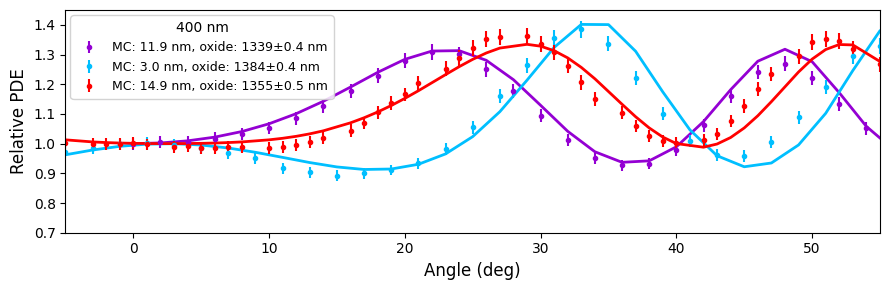
\includegraphics[width=.9\linewidth]{fig-FBK_angular_reduced.png}
\caption{\label{fig:fbk_angularData} Three measurements of FBK device's relative PDE versus angle at 400~nm. Monochromator FWHM (MC width) from each campaign and fit oxide thickness $\tox$ are given in the legend. Other wavelengths are omitted for clarity but are included in the fits.}
\end{figure}

The relative angular PDE for the FBK device was measured in three separate campaigns, with monochromator settings modified for each run. Each campaign yielded slightly different oscillation patterns giving different oxide thicknesses within 2\% of the mean 1358~nm. Thicknesses from the Franta input dataset are within 0.5~nm of the default dataset values. Variance between runs is ascribed to the MC transfer function coupled to the underlying lamp spectrum (see \autoref{sec:measuring_relativePDE}), a systematic requiring further investigation for high resolution ellipsometry. \autoref{fig:fbk_angularData} show the measurement at 400~nm although each campaign and fit contain multiple wavelengths.

% The second and third campaigns extend to -10$^\circ$. A small correction to the angle's zero-point is calculated by assuming the data should be symmetric about $\pm 10^\circ$, resulting in a shift of +2.5 degrees which is applied to the relative transmission fit function. The MC FWHM was mechanically varied for each campaign and is incorporated into the fit procedure. Each campaign yielded slightly different oscillation patterns. A variety of fits were tested using a single oxide thickness and possible experimental nuisance parameters to explain the data (wavelength shifts between runs, angular offsets or MC width). These efforts were unable to produce consistent results, and it was necessary to assign a different oxide thickness to each campaign. Although all oxide thicknesses are within 2\% of the mean value 1358~nm, they are not within fitting uncertainty and the observable oscillation peaks and valleys are clearly inconsistent. The thicknesses using the Franta dataset are within 0.5~nm of the default ones.
 
% \begin{figure}[h]
% \centering
% 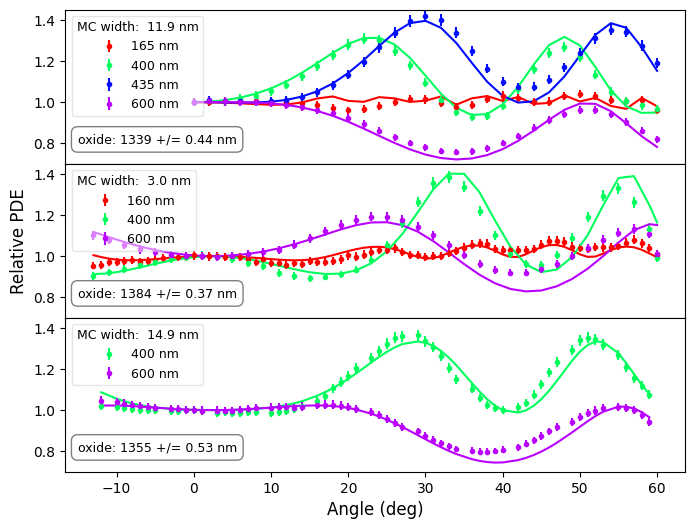
\includegraphics[width=.75\linewidth]{fig-FBK_angular.png}
% \caption{\label{fig:fbk_angularData} Three measurements of FBK device's relative PDE versus angle, fit to extract the oxide thickness. Monochromator FWHM (MC width) was changed for each campaign and are noted in the legends, along with fitted oxide thicknesses displayed in the lower left. The UV data (red) are shifted by an additional wavelength offset of -10~nm (upper) and -15~nm (middle), which is attributed to the spectral non-uniformity of the light source.}
% \end{figure}

% The 160, 165~nm UV data are not included in the fit as we suspect a large spectral uncertainty due to the underlying peak in the deuterium lamp's spectrum. In \autoref{fig:fbk_angularData} the UV fits for 160 and 165~nm are shifted by -10 and 15~nm, respectively, with the intention to demonstrate it is possible to fit the UV data under reasonable assumptions. This campaign provided insight into experimental systematics as the oxide thickness is also derivable from oscillations in $PDE(\lambda)$.

\subsection{Wavelength-dependent PDE for the FBK VUV-HD}
The FBK VUV-HD device's PDE was measured from 350-830~nm at 160~K and 1-6~V overvoltage. Accurate measurement at higher overvoltage was not possible due to an increased rate of correlated avalanches confounding pulse-finding analysis. Data are overlayed with the fit in \autoref{fig:fbk_wlenData}, with inset showing the model extrapolated to longer wavelengths relevant to ExCT. The device parameters derived from the global fits (using the $P_e, P_h$ parameterization) are given in \autoref{tab:fitResults}. The nested $P_e, P_h$ fit produce slightly larger junction geometries. Fitting $PDE(\lambda)$ yielded an oxide thickness of 1358.6~nm, within 1~nm of the angular measurements' mean.

\begin{figure}[htbp]
\centering
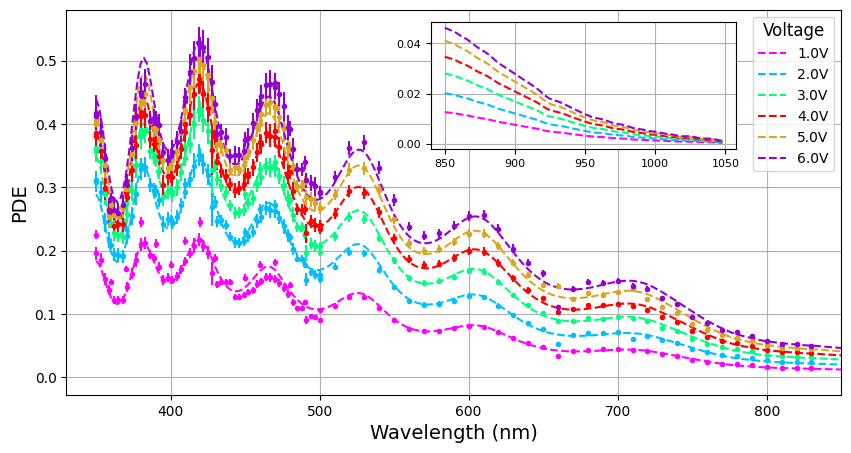
\includegraphics[width=.9\linewidth]{fig-FBK_wavelength_inset_wider.png}
\caption{\label{fig:fbk_wlenData}
FBK data and the global parameterized fit result using the default input dataset. Outlying data points in 1~V curve from the lower resolution wavelength scan can be seen. Inset plot shows PDE extrapolated to 1050~nm. The resulting $P_e$ curves are almost identical to those for HPK, shown in \autoref{fig:hpk_wlen_fit}.}
\end{figure}

\subsection{Reflectivity and oxide layer thickness for the Hamamatsu VUV4}
\label{sec:HPK_Oxide}
For thin oxides, fitting $\tox$ from PDE is difficult as there is weak angular dependence and wavelength response is convolved with internal efficiency. Stronger constraints are available from VUV specular reflectivity data, reported by the nEXO group for two VUV4 devices with different pixel pitch \cite{sipmRef_nexo_guofu}. We fit the data with \autoref{eq:Ref_wave} multiplied by $FF$. The data in \cite{sipmRef_nexo_guofu} is consistently lower by roughly 20-25\%, but for oxide thickness of approximately $\sim 17$~nm the shape agrees well. Different combinations of wavelength and angular data were fit \footnote{The shadowing effect in \autoref{eq-FFtheta} was included in the angular fit, with an extra factor of two on the $\tan\theta$ term as the specularly reflected light is blocked on entry and exit.}, yielding a $\sim$3~nm thicker oxide on the 75~um pitch device than the 50~um pitch device. Uncertain if this difference is by design or variation in fabrication, we take the weighted average fit values as the central value for $\tox$ with the maximum and minimum as the systematic bounds. The identical procedure is carried out using the Franta optical data, which shifted the central value from 17.2~nm to 19.4~nm. Resulting $\tox$ values are listed in \autoref{tab:fit_optics_oxides}.

\begin{table}[h]
\centering
\caption{HPK oxide thicknesses derived from reflectivity data in \cite{sipmRef_nexo_guofu}, for the given input optical dataset. First two columns are the average per device, last column is weighted average and upper/lower limits.
\label{tab:fit_optics_oxides}}
\smallskip
\footnotesize
\renewcommand{\arraystretch}{1.3}  % Default is 1.0
\begin{tabular}{|c|c|c|c|}
    \hline
    \textbf{Input data} & \textbf{50~$\bm{\um}$ pitch} &  \textbf{75~$\bm{\um}$ pitch} & \textbf{Estimated thickness $\bm{(\tox)}$} \\
    \hline
    default & 16.1~nm & 18.8~nm & \makecell{  $17.2^{+2.4}_{-1.3}$~nm } \\
    % \hline
    % Franta (150~K)  & 17.3~nm & 20.8~nm & \makecell{ $19.4^{+1.9}_{-2.7}$~nm  }\\
    \hline
\end{tabular}
\end{table}

\subsection{Wavelength-dependent PDE for the Hamamatsu VUV4}
\begin{figure}[h]
\centering
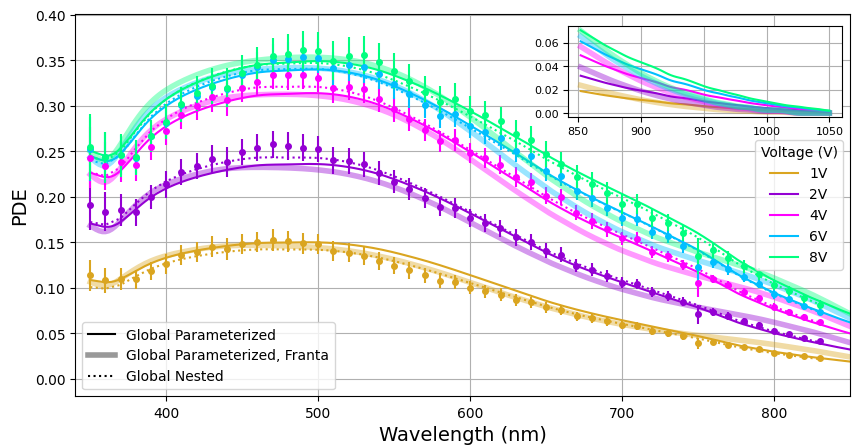
\includegraphics[width=0.8\linewidth]{fig-HPK_pde_wide_inset_noPE.png}
\caption{
    \label{fig:hpk_wlen_fit} The HPK PDE for selected overvoltages is shown, with 3 fits overlayed. The `nested' (unconstrained) $P_e, P_h$ fits perform slightly better near the $\sim$500~nm maximum. At higher overvoltages the Franta fit (thick line) underestimate the PDE in the NIR. Inset shows both parameterized fits extended to 1050~nm, where the Franta prediction drops faster. Avalanche probabilities are given in \autoref{fig:Ph}.}
\end{figure}

The absolute efficiency of the HPK VUV4 device was measured at 163~K from 350-830~nm for overvoltages 1-8~V. Experimental data with model fit, including various $P_e(V), P_h(V)$ curves, are shown in \autoref{fig:hpk_wlen_fit}. Device parameters derived from the global fit are listed in \autoref{tab:fitResults} while different $P_e, P_h$ results are compared in the discussion. Two other fits are shown; one using the input Franta optical dataset and the unconstrained (nested) fit.

The nested fit yields a lower reduced chi-squared with main improvements at lower overvoltage data. Junction parameters are only slightly modified. The global fit was repeated for the systematic uncertainty on oxide thickness $\tox$, listed as percent difference on the central values in \autoref{tab:fitResults}. All parameters were modified by less than 5\% with the exception of $dp^*$ by -13\%, +43\% for the 15.9~nm and 19.6~nm oxide values, respectively, due to larger shifts in UV transmission.

\subsection{Angular dependence of PDE for the Hamamatsu VUV4 - effects of device microstructure}
\begin{figure}[h]
\centering
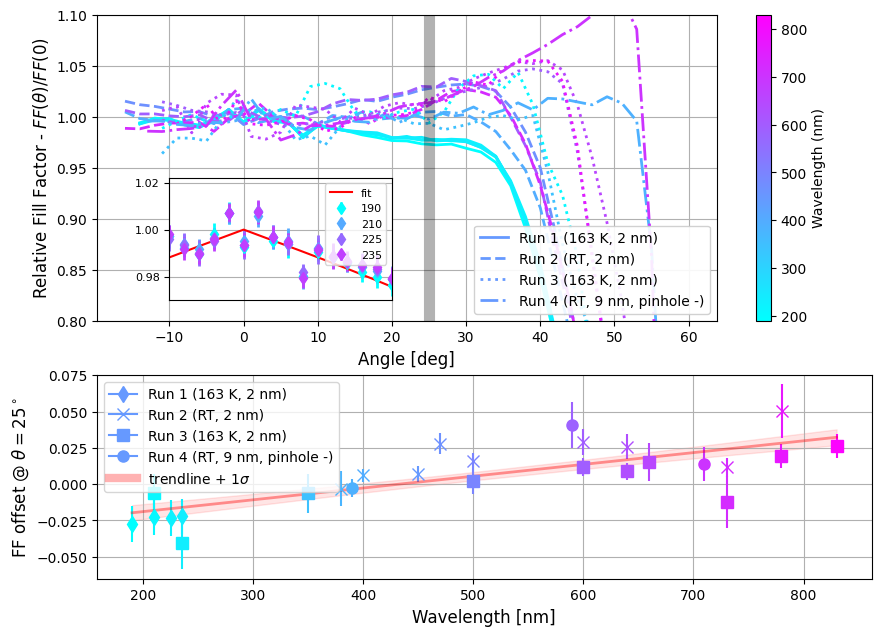
\includegraphics[width=0.7\linewidth]{fig-HPK_angular_FF_sparse_wider.png}
\caption{Upper plot showing $FF(\theta)/FF(0\degree)$, derived from relative PDE data with transmission factored out. Inset shows the UV data with shadowing \autoref{eq-FFtheta} fit for the effective resistor height. The lower plot shows $FF(\theta)/FF_o - 1$ about 25$\deg$ (dark vertical line) versus wavelength. Some experimental data omitted from upper figure for clarity. \label{fig:hpk_angular_ff}}

    % \caption{Some of the angular data is noisy and some curves are not pictured on the upper plot. The inset shows the shadowing fit of the (non-noisy) UV data. The lower plot shows the offset from unity at 25 degrees, showing linearity with wavelength.
\end{figure}

The angular dependence of PDE was measured for the HPK VUV4 device at wavelengths between 190-830~nm. We observed a small discrepancy between the predicted and measured $PDE(\theta)$, assuming $FF$ is fixed with angle. The relative transmission $T(\theta)/T_o$ is removed from the relative angular PDE (\autoref{sec:measuring_relativePDE}), with the subscript denoting the value at normal incidence and $FF_o = 0.6$. The result is a `measured' relative fill factor, $FF(\theta)/FF_o \approx PDE(\theta)\cdot T_o / PDE_o \cdot T(\theta)$ as the internal PDE is independent of AOI. Relative $FF$ is shown in \autoref{fig:hpk_angular_ff} which is not flat. The falloff at high AOI is due to beam containment or device packaging (onset varies with collimator size). The offset of $FF(\theta)/FF_o$ from unity at $25^\circ$ is plotted versus wavelength, showing a monotonic wavelength dependence; in the UV, the effective $FF(\theta)$ is decreasing with angle while for longer wavelengths $FF(\theta)$ increases.

We assume for UV wavelengths the shadowing model (\autoref{sec:ffTheta}) accurately describes the system, as the polysilicon material is highly absorbing and diffraction should be small\footnote{This was estimated by treating the system as a `half-plane diffraction' problem and integrating the total intensity of E field bent below the plane.}. We fit the UV data (190-235~nm, solid lines in \autoref{fig:hpk_angular_ff}) from -15 to 30 degrees for an effective resistor height $h$ with equation \ref{eq-FFtheta}. The fit yields a value $h = 2.6 \pm 0.1$~um and a reduced chi-squared of 1.6, in excellent agreement with AFM measurements performed by the nEXO collaboration\footnote{Acknowledgements to Prabandha Nakarmi, who performed this measurement in 2022} which report a resistor height between 2.5~um and 3~um. Using the upper and lower values of $\tox$ or the Franta dataset all give resistor heights within this range.

\subsection{Variations with fit procedure}
The assumption that $P_e$ saturates to unity was tested for the HPK device. Floating $A_e$ in the parameterized fits yields $A_e = 0.99\pm 0.01$ and the unparameterized (`nested') fit yields $P_e(8\text{V}) = 0.99 \pm 0.01$. For FBK, $P_e(V)$ does not saturate to 1.0; however the data is limited to 6~V preventing definitive conclusions. The nested fit improves fit quality due to the flexibility in $P_e(V)$. For both devices the sequential and global fit parameters agree, other than $P_e(V)$ when a very narrow UV range is used (350-380~nm).

For the VUV4, variation in $dp^*$ with fit method is driven by the the model's significant curvature about $~\sim$360~nm, a product of transmission and $W_p(\lambda)$. Artificially increasing the monochromator's FWHM could not sufficiently reduce this effect. Including longer wavelength PDE increases $P_e$, at the expense of a worse fit in the UV region where an otherwise shallower $dp^*$ and lower $P_e$ flatten the response. For FBK, the parameterized fit forces a deeper $dp^*$ than the nested fit due to the low overvoltage data; $V_e$ is sensitive to the exact breakdown voltage.

Fitting with the Franta dataset significantly worsens the chi-squared by 2-4 times, and results are omitted from \autoref{tab:fitResults}. The lower photoabsorption and shape reduces the n-type region's size by approximately 2 with a correlated increase in $P_h$ given by $V_h = 4.7\pm 0.3$~V and $V_h = 13.7 \pm 0.4$~V, for HPK and FBK respectively. $dp^*$ is reduced to counteract sharper features in UV optical constants.

\begin{table}[h]
\centering
\caption{A table showing fit results from PDE vs wlen for both devices. FBK oxide thickness $\tox$ is fit from the PDE while the HPK value is independently derived from reflectivity data in \cite{sipmRef_nexo_guofu}. Results listed are from a global fit with $P_e, P_h$ parameterized as $1-e^{-V/V_{e,h}}$, global fit for HPK, and others discussed in the text. The FBK oxide is almost 100 times thicker than HPK, and the junction smaller with a different asymmetric shape. Both devices show similar avalanche probabilities.
\label{tab:fitResults}
}
\smallskip
{\scriptsize
\setlength{\tabcolsep}{2.5pt}
\renewcommand{\arraystretch}{2.5}  % Default is 1.0
\begin{tabular}{|c|c|c|c|c|c|c|c|c|}
    \hline
    \textbf{Device} & \textbf{Fit} & $\bm{\tox}$ (nm) & $\bm{dp^*}$ (nm) & $\bm{X_{PN}}$ (um) & $\bm{dw^*}$ (um) & $\bm{V_e}$ or $\bm{P_e(8\text{V})}$ & $\bm{V_h}$ or $\bm{P_h(8\text{V})}$ & $\bm{\chi^2/\nu}$ \\
    
    \hline

    %% old data w mistake in code
    % \makecell[c]{FBK\\VUV-HD} & Parameterized & 1358.9 $\pm$ 0.2  & $0.90 \pm 0.06$ & $0.51 \pm 0.01$ & $8.39 \pm 0.13$ & $1.83 \pm 0.01$ & $18.90 \pm 0.27$ &  $\nicefrac{1734}{588}$  \\
    \multirow{2}{*}{\makecell[c]{FBK\\VUV-HD}} & Parameterized & 1358.9 $\pm$ 0.2  & $2.73 \pm 0.06$ & $0.42 \pm 0.01$ & $8.03 \pm 0.12$ & $1.87 \pm 0.01$ & $20.1 \pm 0.26$ & $\nicefrac{2703}{588}$  \\
    
    \cline{2-9}
    
     & Nested & 1358.9 $\pm$ 0.2  & $1.1 \pm 0.07$ & $0.50 \pm 0.01$ & $8.43 \pm 0.13$ & $0.88 \pm 0.003$ & $0.23 \pm 0.002$ &  $\nicefrac{1464}{578}$  \\
    \hline
    
    \multirow{2}{*}{\makecell[c]{HPK\\VUV4}} & Parameterized &
    \multirow{2}{*}{\makecell{$17.20^{+2.43}_{-1.31}$}} & 
    \makecell{$1.03 \pm 0.24$ \\ \scriptsize{$+37\%, -19\%$}} &
    \makecell{$2.35 \pm 0.07$ \\ \tiny{$+1.7\%, -0.8\%$}} & 
    \makecell{$13.6 \pm 0.8$ \\ \tiny{$+3.7\%, -1.7\%$}} &
    \makecell{$1.80 \pm 0.022$ \\ \tiny{$+1.7\%, -1.1\%$}} & 
    \makecell{$16.76 \pm 1.21$ \\ \tiny{$+5.1\%, -2.4\%$}} & $\nicefrac{188}{387}$ \\
    \cline{2-2} \cline{4-9}
    
     & Nested &  & 
    $1.31 \pm 0.26$ & $2.08 \pm 0.08$ & 
    $12.4 \pm 0.6$ & $0.99 \pm 0.01$ & $0.41\pm 0.01$ & $\nicefrac{107}{373}$ \\
    
    \hline
    
\end{tabular}
} % end of text size
\end{table}

%% Pe values dont agree perfectly. we learned that you have to know your Vbr `bias' well to use step 3A. Still no Ve values are as low as fits allow so our other PDE terms probably high

% ---- other fit stuff ----
% Allowing $A_e = 0.85$ compensates for overestimate in UV, providing a better fit but is not truly physical; UV $PDE(V)$ matches the shape of the independently measured $P_e(V)$ which rises above 6~V. As such, $P_e$ saturates to a value at least higher than $P_e(6V)=0.88$. Decreasing the $FF$ brings fit results into better agreement with $P_e$ measurements and expectation $A_e \rightarrow 1.0$.

% For either device results from the global and sequential fits agree, with the caveat that the UV wavelength's upper limit is 420~nm (HPK) and 400~nm (FBK) to fit $dp^*$ and $V_e$ (step 3B in \autoref{tab:fitting_procedure}). For HPK restricting the UV fit to 350-380~nm retains agreement other than $dp^*$ coming into tension. Setting $P_e = 1.0$ (step 2 in \autoref{tab:fitting_procedure}) increases $dp^*$ out of agreement.

% Variance in $dp^*$ between procedures means the $P_e$ parameterization is inaccurate for lower voltages (meaning the high-V $dp^*$ is more accurate) or inaccuracy of the predicted UV transmission (all-V $dp^*$ is more accurate).